In this project I have investigated a system of $N=$ 2, 6 and 12 electrons, where $N$ is the number of particles. It is a so-called closed shell-system. The Hamiltonian used to model this system is

\begin{equation}
\label{eq:finalH}
\hat{H}=\sum_{i=1}^{N} \left(  -\frac{1}{2} \nabla_i^2 + \frac{1}{2} \omega^2r_i^2  \right)+\sum_{i<j}\frac{1}{r_{ij}},
\end{equation}
where 
$$\hat{H}_0=\sum_{i=1}^{N} \left(  -\frac{1}{2} \nabla_i^2 + \frac{1}{2} \omega^2r_i^2  \right)$$
is the single particle part and

\begin{equation}\label{eq:hamilton_interaction}
\hat{H}_1=\sum_{i<j}\frac{1}{r_{ij}},
\end{equation}

represent the interaction potential between particles. The Hamiltonian is written in atomic units, which implies that $\hbar = 1, m= 1$, the unit of length is $a_0 = \nicefrac{4 \pi \epsilon_0 \hbar^2}{m_e e^2}$ and the unit of energy is $E_h = \nicefrac{\hbar^2}{m_e a_0^2}$.  In Eq. \ref{eq:hamilton_interaction} $r_{ij}=\vert \bm{r}_i-\bm{r}_j\vert= \sqrt{(x_i-x_j)^2 + (y_i-y_j)^2}$ and in Eq. \ref{eq:finalH} $\omega$ is the oscillator frequency or the trap frequency.

\subsection{Two particle system}

The single particle wave function in two dimensions is
\begin{equation}\label{eq:single_particle_wf}
\phi_{n_x,n_y}(x,y) = A H_{n_x}(\sqrt{\omega}x)H_{n_y}(\sqrt{\omega}y)\exp{(-\omega(x^2+y^2)/2}.
\end{equation}
where the functions $H_{n_x}(\sqrt{\omega}x)$ are Hermite polynomials,  while $A$ is a normalization constant. The relevant Hermite polynomials in this project are listed in Appendix \ref{app:hermite_and_derivatives}.

For the lowest-lying state, $E_{00}$  (see Fig. \ref{fig:states}), we have $n_x=n_y=0$ and an energy $\epsilon_{n_x,n_y}=\omega(n_x+n_y+1) = \omega$, the total energy of the lowest-lying state is hence $2\omega$ because there is, due to Pauli's exclusion principle, room for two electrons with opposite spins. The total spin of the ground state for the system with two electron is therfore zero. The same applies for all closed shell systems in the ground state because the filled states all have two electrons with opposite spins that cancel each other. The energies of the other full-shell systems that include an increasing number of states are listed in Appendix \ref{app:energies}. 

\begin{figure}[H]
\center
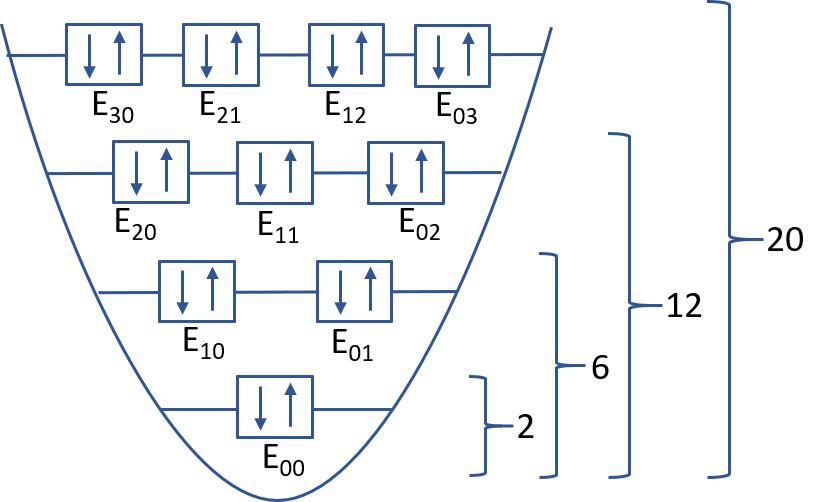
\includegraphics[width=0.6\linewidth]{../Results/states}\caption{Illustration of the different electron states in a harmonic oscillator trap. The numbers $E_{ij}$ represent the different single-particle states and the states at the same level have the same energy. The arrows show that two electrons with opposite spins can occupy the same state. On the right the full shell systems with the according number of particles are pointed out.}\label{fig:states}
\end{figure}

The expectation value can be found by solving the equation

\begin{equation}\label{eq:expectation_energy}
   \langle E_L \rangle =
   \frac{\int d\bm{r}_1d\bm{r}_2\psi^{\ast}_T(\bm{r}_1,\bm{r}_2)\hat{H}(\bm{r}_1,\bm{r}_2)\psi_T(\bm{r}_1,\bm{r}_2)}
        {\int d\bm{r}_1d\bm{r}_2\psi^{\ast}_T(\bm{r}_1,\bm{r}_2)\psi_T(\bm{r}_1,\bm{r}_2)}.
\end{equation}

We use Variational Monte Carlo (VMC) methods to evaluate the Eq. \ref{eq:expectation_energy} \cite{project1}. The exact wave function for two not interacting electrons in the ground state is given by

\begin{equation*}
\Phi(\bm{r}_1,\bm{r}_2) = C\exp{\left(-\omega(r_1^2+r_2^2)/2\right)},
\end{equation*}

where $r_i = \sqrt{x_i^2+y_i^2}$ and C is a normalization constant. The trial wave function we use for the not interacting case is 
\begin{equation}\label{eq:trial_wf_not_interacing}
\Phi(\bm{r}_1,\bm{r}_2) = C\exp{\left(-\alpha\omega(r_1^2+r_2^2)/2\right)}.
\end{equation}

with the parameter $\alpha$. From the exact wave function we know that $\alpha = 1$ for the situation without interaction. On the other hand, for the interacting case, the trial wave function for the two-electron system is

\begin{equation}
   \psi_{T}(\bm{r}_1,\bm{r}_2) = 
   C\exp{\left(-\alpha\omega(r_1^2+r_2^2)/2\right)}
   \exp{\left(\frac{ar_{12}}{(1+\beta r_{12})}\right)}, 
\label{eq:trial_interacting}
\end{equation}

where we introduce another parameter, $\beta$, and a spin factor, $a$. $a$ is 1 when the two electrons have anti-parallel spins and $1/3$ when they have the parallel spins (this is not relevant before one includes more than two particles to the system, as can be seen from Fig. \ref{fig:states}). This trial wave function is not the exact wave function, hence the simulation can only approximate the exact values for the ground state energy.

\subsection{More particles}

Since we are looking at closed shell systems, the next amount of particles are six. We can see this from Fig. \ref{fig:states}, there are room for two electrons with opposite spin in the states here named $E_{01}$ and $E_{10}$, in addition to the two in the lowest lying state. The trial wave function is now given by

\begin{equation}
   \psi_{T}(\bm{r}_1,\bm{r}_2,\dots, \bm{r}_6) = 
   Det\left(\phi_{1}(\bm{r}_1),\phi_{2}(\bm{r}_2),
   \dots,\phi_{6}(\bm{r}_6)\right)
   \prod_{i<j}^{6}\exp{\left(\frac{a r_{ij}}{(1+\beta r_{ij})}\right)},
\end{equation}

where 
$$ Det\left(\phi_{1}(\bm{r}_1),\phi_{2}(\bm{r}_2),
   \dots,\phi_{6}(\bm{r}_6)\right) =  \begin{vmatrix}
  \phi_{1}(\bm{r}_1) & \phi_{2}(\bm{r}_1) & \cdots & \phi_{6}(\bm{r}_1) \\
  \phi_{1}(\bm{r}_2) & \phi_{2}(\bm{r}_2) & \cdots & \phi_{6}(\bm{r}_2) \\
  \vdots  & \vdots  & \ddots & \vdots  \\
  \phi_{1}(\bm{r}_6) & \phi_{2}(\bm{r}_6) & \cdots & \phi_{6}(\bm{r}_6) 
\end{vmatrix}$$
is the Slater determinant. This determinant occurs because electrons are indistinguishable particles and their wave function is hence antisymmetric. The functions, $\phi_{i}(\bm{r}_j)$,  are given by Eq. \ref{eq:single_particle_wf} and the notation is explained in Tab. \ref{tab:notation_wavefunctions}. 

\begin{table}[H]\caption{The relation between the notation used in the determinant (left) compared to Eq. \ref{eq:single_particle_wf} (right). }\label{tab:notation_wavefunctions}
\large
\center
\begin{tabular}{l|l} 
$\phi_{1}$ & $\phi_{n_x=0, n_y=0}$\\
$\phi_{2}$ & $\phi_{n_x=0, n_y=0}$\\
$\phi_{3}$ & $\phi_{n_x=1, n_y=0}$\\
$\phi_{4}$ & $\phi_{n_x=1, n_y=0}$\\
$\phi_{5}$ & $\phi_{n_x=0, n_y=1}$\\
$\phi_{6}$ & $\phi_{n_x=0, n_y=1}$\\
\end{tabular}
\begin{tabular}{c}
$\,$
\end{tabular}
\begin{tabular}{l|l} 
$\phi_{7}$ & $\phi_{n_x=2, n_y=0}$\\
$\phi_{8}$ & $\phi_{n_x=2, n_y=0}$\\
$\phi_{9}$ & $\phi_{n_x=1, n_y=1}$\\
$\phi_{10}$ & $\phi_{n_x=1, n_y=1}$\\
$\phi_{11}$ & $\phi_{n_x=0, n_y=2}$\\
$\phi_{12}$ & $\phi_{n_x=0, n_y=2}$\\
\end{tabular}
\end{table}

Similarly if we include another shell in our system we get 12 particles and the trial wave function is 

\begin{equation}
   \psi_{T}(\bm{r}_1,\bm{r}_2, \dots,\bm{r}_{12}) = 
   Det\left(\phi_{1}(\bm{r}_1),\phi_{2}(\bm{r}_2),
   \dots,\phi_{12}(\bm{r}_{12})\right)
   \prod_{i<j}^{12}\exp{\left(\frac{ar_{ij}}{(1+\beta r_{ij})}\right)}.
\end{equation}

The determinant have the same structure as for six particles and the relation to the single-particle wave functions are shown in Tab. \ref{tab:notation_wavefunctions}.

\subsection{Relevant topics for this project}

For an explanation of the VMC method, sampling methods, optimization and gradient descent methods, statistical analysis and resampling techniques used in this project see the theory part of Project 1 \cite{project1}. However, below is some topics that are explained in further detail or new to this project. 

\subsubsection{Gradient descent - two parameters}

In this project the gradient descent method also known as steepest descent method  was used to evaluate the parameters that makes the trial wave function approximate the ground state wave function \cite{gradient_descent}. Compared to Project 1, there are two parameters to be evaluated. The derivative of the trial wave function with regards to the parameter $\alpha$ is 

\begin{equation}\label{eq:alpha_derivative}
\frac{\frac{\partial \psi_T}{\partial \alpha}}{\psi_T} = -\frac{\omega}{2}\sum_i^N r_i^2
\end{equation}
and $\beta$ is
\begin{equation}\label{eq:beta_derivative}
\frac{\frac{\partial \psi_T}{\partial \beta}}{\psi_T} = - \sum_{i<j}^N \frac{a_{ij}r_{ij}^2}{(1+\beta r_{ij})^2}.
\end{equation}

The derivative used in the gradient descent method is 

\begin{equation}
\frac{\partial \left< E_L \right>}{\partial \alpha} = 2  \left( \left<\frac{\bar{\psi_T^{\alpha}}}{\psi_T}E_L\right> -\left<\frac{\bar{\psi_T^{\alpha}}}{\psi_T}\right>\left<E_L\right> \right)
\end{equation}
where $\left<\frac{\bar{\psi_T^{\alpha}}}{\psi_T}\right>$ is the expectation value of Eq. \ref{eq:alpha_derivative} and $\left<\frac{\bar{\psi_T^{\alpha}}}{\psi_T}E_L\right>$ is the expectation value of Eq. \ref{eq:alpha_derivative} multiplied with the local energy, and the same applies for the parameter $\beta$ (except using Eq. \ref{eq:beta_derivative}). 

\subsubsection{One-body density}

The radial one-body density is a measure of the spacial distribution of the electrons with respect to the distance from the origin of the harmonic oscillator trap. To calculate the radial one-body density, I sampled the position of the electrons at each accepted step in the MC cycles. To sample the positions, the distance from the origin to a set cut-off length was separated into bins with a length $\Delta r$. For every Monte Carlo step, the distance between the electron's position and the origin was calculated, and the bin that corresponded to the current distance got a count. In the end, one has an array corresponding to the different bins with counts corresponding to how many times an electron was found to have that particular distance to the origin. This array is normalized by dividing by the number of Monte Carlo steps. However, to get the density, one has to divide the number in the bins with the area or volume the bin represents. Because this project involve a two-dimensional problem, and I wanted to calculate the radial one-body density, I divided bin $i$ with the area $ A = \pi (r_i+\Delta r)^2 - \pi r_i^2$ where $r_i$ is distance from the origin to bin $i$. This method to calculate the radial one-body density was found in Ref. \cite{Evens_master}.

\subsubsection{Virial theorem}

The virial theorem gives a relation between the time-average total kinetic energy, $\left<T\right>$, and the time-average external potential energy, $\left<V_{ext}\right>$, that is

\begin{equation}\label{eq:virial_theorem}
2\left< T\right> = n\left< V_{ext}\right>
\end{equation}

where $V(r) = Br^n$. In our case, when interaction is not included, $n = 2$ from the external potential term in Eq. \ref{eq:finalH}, and therefore the average kinetic energy should be equal to the average potential energy. This can be used as a test to see if the simulations executed are correct. 

\subsubsection{Trap frequency}

The trap frequency changes the external potential felt by the electrons. Figure \ref{fig:harmonic_oscillator_potential} shows how a larger trap frequency, $\omega$, results in a narrower external potential. In this narrow harmonic oscillator trap, the electrons are forced to be closer to each other. Later, I look at how $\omega$ affects the energy when the electrons are interacting with each other through the potential given in Eq. \ref{eq:hamilton_interaction}.

\begin{figure}[H]
\center
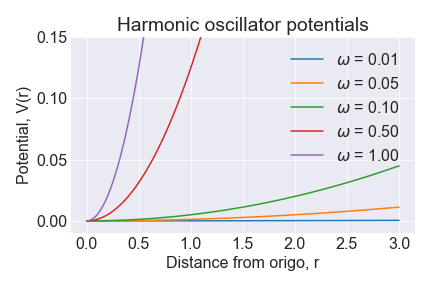
\includegraphics[width=0.7\linewidth]{../Results/harmonic_oscialltor_potentials}\caption{Illustration of how the potential changes when the trap frequency changes. }\label{fig:harmonic_oscillator_potential}
\end{figure}

\subsubsection{Evaluating the error}

To evaluate the error of the calculated expectation energy one can use the standard error of the mean (SEM)
\begin{equation}
\text{SEM} = \frac{\sigma}{\sqrt{N}}
\end{equation}
where $N$ is the number of observations, in our case the number of Monte Carlo (MC) cycles. One can easily see that an increased number MC cycles will decrease the SEM.

\subsection{The program}

The program is found at this \href{https://github.com/vildemjo/vmc_fermions}{GitHub} repository and includes comments to describe the code, but below are some general aspects of the program.

\subsubsection{Initialization}

First the different parts of the program is initialized based on what Hamiltonian that is used and what wave function is used. In this program, one can choose a Hamiltonian with and without interaction (\texttt{InteractionHarmonicOscillator} and \texttt{HarmonicOscillator}, respectively), and accordingly, a wave function with and without a Jastrow factor (\texttt{SlaterDeterminantInteraction} and \texttt{Slaterdeterminant}, respectively). Thereafter, the initial state is set up. The particles are distributed randomly after a set distribution. Two different distributions are used and chosen based on the sampling method. For importance sampling a Gaussian distribution is used (\texttt{GaussainDistribution}) and for brute force sampling a random uniform distribution is used (\texttt{RandomUniform}). This initialization reflects in the way the sampling of new positions are made by the sampling method, which is explained in project 1 \cite{project1}.

\subsubsection{Metropolis steps}

After the initialization the particles are moved one by one, chosen at random, and the new position is found through the sampling method. The metropolis ratio is calculated to determine whether the step is accepted or not. The metropolis ratio is also determined by the sampling method. If the step is accepted, the energy is sampled and if not, the former energy is sampled again. This is continued until all Monte Carlo (MC) cycles have finished. 

\subsubsection{Sampling}

In this program one can choose to sample all local energies for all MC cycles. This makes it possible to performed resampling techniques on the dataset to improve estimate of the error by estimating the correlation between the different metropolis steps, i.e. the samples made of the local energy. For the other outputs, e.g. kinetic, potential and interaction energy and the mean distance, the average is calculated based on the sum of all the sampled values by dividing by the number of MC cycles.

\subsection{Improving performance and efficiency}

An important part of numerical simulations is computational performance and efficiency. Below are some topics related to this.

\subsubsection{Vectorization}

Compliers can optimize the code in different ways and one of them is called vectorization. With vectorization more of the memory is used simultaneously and operations are executed on vectors instead of scalars. This makes the code more efficient and can reduce the CPU time of the code. To include vectorization in my program I added

\begin{lstlisting}
set(CMAKE_CXX_FLAGS_RELEASE "-O3")
\end{lstlisting}

in \texttt{CMakeLists}.

\subsubsection{Parallelizing}

Parallelizing the code is doing operations in parallel instead of sequentially. One can use different methods to parallelize code and combine different methods like MPI and openMP. The different methods can be easy or difficult to implement based on how much you control the the transfer of information between different processes. 

In this case the parallelization needed is very simple. We want more MC cycles in less time. In this project I chose to parallelize using a Makefile and cmake. I ran the whole executable with different seeds for the random number generator and different file names to save all the local energies in four different threads on my own personal computer which is a quad-core laptop.

\subsubsection{Reducing computational cost}

An important part of making the program more efficient is to reduce the number of floating point operations (flops) by implementing a smart code and use expressions for ratios, e.g. the metropolis ratio. 

In this particular project one can do many different things to make the code more efficient. The first thing is to split the Slater determinant into a spin-up determinant and a spin down determinant. By doing this one only have to update either of them when a spin up/spin down particle is moved. How this is done is explained further in Appendix \ref{app:efficient_SD}. Another method to reduce flops is to find an expression for the metropolis ratio, instead of calculating individual parts and afterwards calculate the ratio. This is explained in Appendix \ref{app:efficient_R}. Other implementations are to updating the inverse instead of calculating the inverse for every step (see Appendix \ref{app:inverse_update}). All of these changes results in another structure when performing the metropolis step (when importance sampling is used):
\begin{itemize}
\item Pick particle at random and find new position
\item Update Slater determinant row (spin up or spin down one based on the particle that was picked)
\item Calculate both old and new quantum force (gradient in a specific position) using the old inverse Slater determinant (see Appendix \ref{app:gradients_double_derivatives}).
\item Calculate the metropolis ratio using the new Slater determinant and the old inverse determinant.
\item Update the inverse Slater determinant (only spin up or spin down one based on the particle that was moved) only if the move is accepted. 
\end{itemize}
Using this structure saves many flops since the inverse Slater determinant do not have to be calculated or updated at all if the move is not accepted and, as an example, updating the inverse Slater determinant takes $O(N^2)$ instead of $O(N^3)$ when the inverse is calculated. 